%=======================================================================
%  CSE 438 — Digital Image Processing · Assignment Part B
%  Two-column IEEE conference format (mandated by the assignment brief)
%  Compile: pdflatex report.tex   (Overleaf: set compiler to pdfLaTeX)
%=======================================================================
\documentclass[conference]{IEEEtran}
\IEEEoverridecommandlockouts

\usepackage{cite}
\usepackage{amsmath,amssymb}
\usepackage{graphicx}
\usepackage{booktabs}
\usepackage{array}
\usepackage{xcolor}
\usepackage[hidelinks]{hyperref}
\graphicspath{{figures/}}

\newcommand{\best}[1]{\textbf{#1}}

% --- tighter float + caption spacing (16 floats; recovers ~2 in of column space) ---
\setlength{\textfloatsep}{6pt plus 2pt minus 2pt}
\setlength{\floatsep}{6pt plus 2pt minus 2pt}
\setlength{\intextsep}{6pt plus 2pt minus 2pt}
\setlength{\dbltextfloatsep}{6pt plus 2pt minus 2pt}
\setlength{\abovecaptionskip}{3pt}
\setlength{\belowcaptionskip}{0pt}

\begin{document}

%=========================== 6.1 TITLE / AUTHORS ========================
\title{A Controlled Comparison of Four Self-Supervised Pretext Tasks\\
for Label-Efficient Liver and Tumour Segmentation}

\author{
\IEEEauthorblockN{Md.\ Asif Hossain (2022-3-60-007) \quad
                  Nabil Subhan (2022-3-60-063) \quad
                  K M Nudar (2022-3-60-234)}
\IEEEauthorblockA{Group 01 \quad CSE 438 --- Digital Image Processing \quad
Dept.\ of CSE, East West University, Dhaka, Bangladesh\\
Dataset: LiTS $256\times256$ (Liver Tumour Segmentation Challenge)}
}

\maketitle

%=========================== 6.1 ABSTRACT ==============================
\begin{abstract}
Pixel-level annotation is the dominant cost in medical image segmentation, so a
central question is how much labelled data remains necessary once an encoder has
learned good visual representations without labels. We answer this question under
a controlled protocol: the dataset, the decoder head, the loss, the optimiser and
the label budget are all held fixed, and \emph{only} the self-supervised pretext
task is varied. Four encoders --- SimCLR (contrastive), BYOL (negative-free
self-prediction), MAE (masked reconstruction) and DINOv2 (self-distillation) ---
are pretrained for 50 epochs on 13{,}447 unlabelled CT slices, fitted with the
ASPP decoder identified as best in Part~A, and fine-tuned for 50 epochs on only
2{,}553 labelled slices, i.e.\ \textbf{19\% of the labels} used by the fully
supervised baseline. Using this fifth of the annotations, the methods recover
93.8--101.0\% of the supervised baseline mIoU. DINOv2 is strongest (mIoU 0.776;
0.749 without test-based checkpoint selection) and exceeds full supervision on
the minority tumour class (IoU 0.463 vs.\ 0.407). MAE inverts the pattern,
achieving the best liver IoU (0.882) but the worst tumour IoU (0.287), showing
that the pretext objective determines \emph{which} structures a representation
encodes, not merely how good it is.
\end{abstract}

\begin{IEEEkeywords}
self-supervised learning, semantic segmentation, label efficiency, computed
tomography, DINOv2, masked autoencoders, contrastive learning
\end{IEEEkeywords}

%=========================== 6.2 INTRODUCTION ==========================
\section{Introduction}

Semantic segmentation assigns a class label to every pixel of an image. In the
medical domain this is the enabling step for volumetry, lesion tracking and
treatment planning, but it is also where the cost sits: a segmentation mask must
be drawn by a trained radiologist, slice by slice, whereas the images themselves
accumulate for free in any hospital archive. Any method that converts abundant
\emph{unlabelled} images into segmentation accuracy therefore has direct
practical value.

Self-supervised learning (SSL) offers exactly this trade. Instead of class
labels, an SSL encoder is trained on a \emph{pretext task} constructed from the
images alone --- matching two augmented views, predicting one view's
representation from another, reconstructing deliberately hidden pixels, or
matching a teacher network's output distribution. Only afterwards, and with far
fewer labels, is the encoder adapted to the downstream task.

Part~A of this assignment established the supervised reference point. Three
architecturally distinct segmentation models --- DeepLabV3-ResNet50,
SegFormer-B0 and YOLOv26-sem --- were benchmarked on the LiTS dataset under one
identical recipe and a leakage-safe, volume-grouped split. DeepLabV3-ResNet50
won, reaching a test mIoU of \textbf{0.768} while training on the full
13{,}447-slice labelled training split, and its ASPP (Atrous Spatial Pyramid
Pooling) head was therefore identified as the best-performing decoder design.
Part~B reuses that dataset, that split and that decoder, and replaces full
supervision with self-supervised pretraining followed by fine-tuning on a much
smaller labelled subset.

The contribution of this report is a \emph{controlled} comparison. Because the
dataset, decoder, loss, optimiser schedule and label budget are identical across
all four methods, any difference in downstream accuracy is attributable to the
pretext task itself. Liver/tumour segmentation is the measurement instrument
rather than the objective: the tumour class occupies only $0.13\%$ of pixels,
which makes it an unusually sensitive probe of representation quality.

%=========================== 6.3 DATASET & SPLIT =======================
\section{Dataset and Split}

\subsection{Dataset}
We use the LiTS $256\times256$ derivative of the Liver Tumour Segmentation
Challenge~\cite{lits}: 131 patient CT volumes rendered as 58{,}638 axial slices.
Each slice is supplied with two separate binary masks (liver and tumour), which
we fuse into a single class-index label with tumour taking precedence,
\[
  y(x)=\begin{cases}
    2 & \text{tumour}\\
    1 & \text{liver, not tumour}\\
    0 & \text{background,}
  \end{cases}
\]
giving three classes. The distribution is severely imbalanced: background
$97.67\%$, liver $2.20\%$, tumour $0.13\%$. Following Part~A we retain only
slices containing liver or tumour and feed the network a \emph{2.5D} input, i.e.\
three channels formed from the adjacent slices $[i-1,\,i,\,i+1]$, which supplies
volumetric context without leaving the source volume.

\subsection{Reuse of the Part-A split}
The leakage-safe split produced in Part~A is loaded \emph{unmodified}; no
re-splitting, re-shuffling or new sub-pooling was performed. The split is grouped
\emph{by patient volume}, which matters because adjacent slices of one volume are
near-duplicates (mean perceptual-hash Hamming distance $\approx 1.9$ within a
volume versus $\approx 14.2$ across volumes); a per-slice split would place the
same patient in both training and test data. We verified the reuse in two ways:
the three volume sets were asserted to be pairwise disjoint, and a SHA-256
fingerprint of each sorted slice list was printed as a provenance stamp shared by
all method notebooks.

\begin{table}[t]
\caption{Split roles inherited from Part~A. The image counts are unchanged; only
the \emph{role} of each split differs in Part~B.}
\label{tab:split}
\centering
\resizebox{\columnwidth}{!}{%
\begin{tabular}{llrr}
\toprule
Part-A split & Role in Part~B & Volumes & Slices\\
\midrule
Train      & Unlabelled SSL pretraining      & 92 & 13{,}447\\
Validation & Labelled fine-tuning            & 20 & 2{,}553\\
Test       & Monitoring \emph{and} evaluation & 19 & 3{,}158\\
\bottomrule
\end{tabular}}
\end{table}

\begin{figure}[t]
\centering
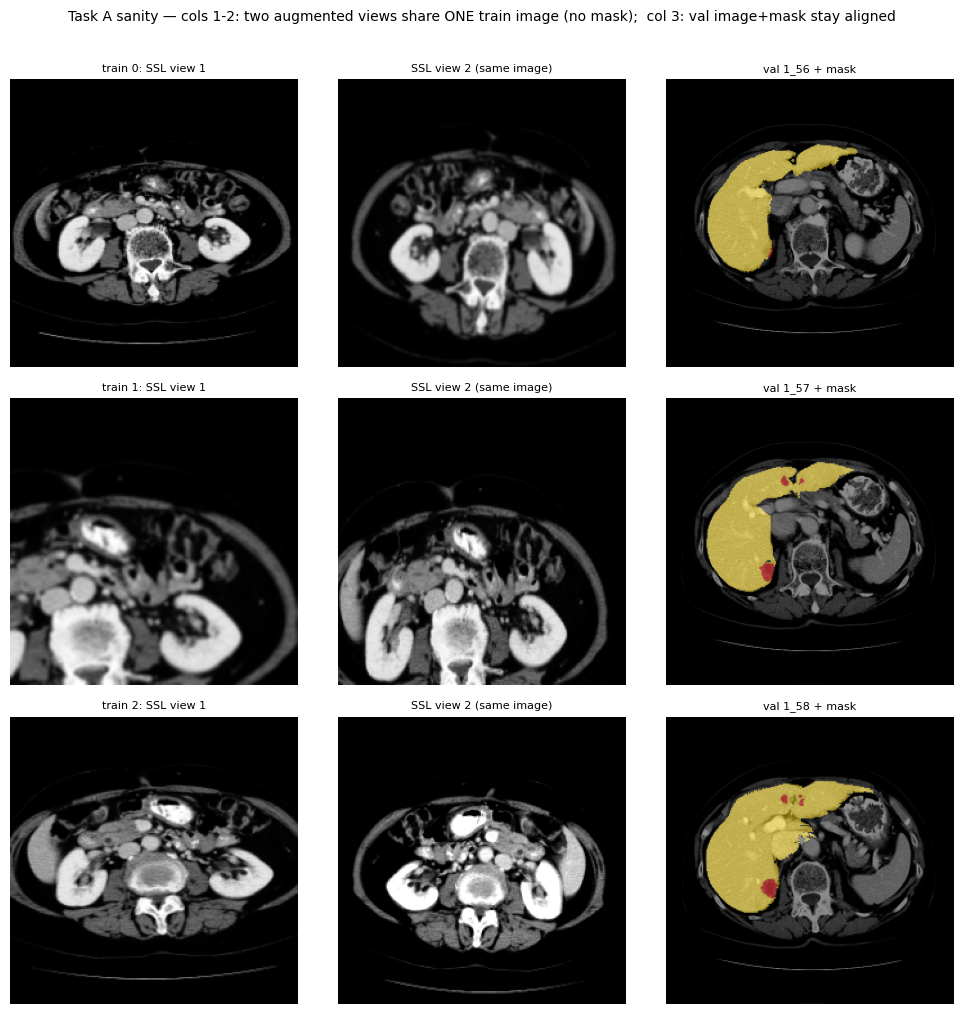
\includegraphics[width=0.56\columnwidth]{sanity_grid.png}
\caption{Task~A sanity check. Columns~1--2: two augmented views of the same
unlabelled training slice (no mask). Column~3: a labelled slice with its fused
mask overlay (liver gold, tumour red).}
\label{fig:sanity}
\end{figure}

Fig.~\ref{fig:sanity} is the Task~A sanity check, confirming both pipelines were
correctly wired before any training. Table~\ref{tab:split} gives the role mapping
and exact counts. The
label-efficiency ratio that governs the whole study is therefore
\[
  \frac{N_{\text{val}}}{N_{\text{train}}}=\frac{2{,}553}{13{,}447}=0.190,
\]
i.e.\ every SSL model is fine-tuned on \textbf{19\%} of the labels the Part-A
baseline consumed.

\subsection{The test split serves a double role}
\label{sec:doublerole}
Following the assignment protocol, the test split is used \emph{twice}: to monitor
fine-tuning and select the best checkpoint, and afterwards to report final
metrics. This is a deliberate simplification --- the labelled set is already
small, and carving out a fourth split would leave too little data to fine-tune on
--- but it is a genuine departure from strict practice, in which a test set is
touched exactly once.

We therefore quantify the resulting optimism rather than presenting the numbers as
if the test set were untouched. Selecting the best of 50 test evaluations returns
the maximum of 50 noisy measurements, which is biased upward. Our per-epoch logs
make the noise explicit: DINOv2's test mIoU moves between 0.694 (epoch~5) and
0.776 (epoch~13) while its \emph{stable} level over the final ten epochs averages
0.750. Accordingly we report both the selected-checkpoint metric and the
epoch-50 metric, which involves no test-based selection; the gap between them is
the selection bias and ranges from $+0.011$ to $+0.032$ mIoU
(Table~\ref{tab:results}). The Part-A baseline does \emph{not} carry this bias, as
it selected on a separate validation split. The correct remedy, given more
labelled data, would be a fourth truly held-out slice of the dataset.

%=========================== 6.4 METHODOLOGY ===========================
\section{Methodology}

All four methods share the pipeline
\begin{equation*}
\begin{aligned}
\text{image}\;&\rightarrow\;\text{SSL encoder}\;\rightarrow\;\text{dense features}\\
             &\rightarrow\;\text{ASPP decoder}\;\rightarrow\;\text{per-pixel class},
\end{aligned}
\end{equation*}
in which only the encoder and its pretext task change.

\subsection{Pretext tasks}

\textbf{SimCLR (contrastive)}~\cite{simclr}\textbf{.} Two augmented views of the
same slice form a positive pair; all other images in the batch are negatives. The
NT-Xent objective
\[
\ell_{i,j}=-\log\frac{\exp(\mathrm{sim}(z_i,z_j)/\tau)}
                     {\sum_{k\neq i}\exp(\mathrm{sim}(z_i,z_k)/\tau)}
\]
is minimised with temperature $\tau=0.2$ and a two-layer projection head
($2048\!\to\!512\!\to\!128$). Because CT slices are effectively grayscale, colour
jitter is deliberately mild; the crop and flip carry the invariance.

\textbf{BYOL (negative-free)}~\cite{byol}\textbf{.} An online network predicts the
projection produced by an exponential-moving-average (EMA) target network from a
differently augmented view, with the symmetric loss $2-2\cos(p,z)$ and
stop-gradient on the target. No negatives are required. The EMA momentum follows a
cosine schedule from $0.996$ to $1$.

\textbf{MAE (masked reconstruction)}~\cite{mae}\textbf{.} $75\%$ of $16\times16$
patches are masked; the encoder sees the corrupted image and a lightweight
transposed-convolution decoder reconstructs the original intensities, with the
loss computed \emph{only over masked pixels}. Following the course reference
implementation we use a ResNet-50 encoder rather than a ViT, so that the
pretrained weights transfer directly into the DeepLabV3 backbone without an
adapter --- this keeps the transfer architecturally exact.

\textbf{DINOv2 (self-distillation)}~\cite{dinov2,dino}\textbf{.} A student
ViT-S/14 matches the output distribution of an EMA teacher over a multi-crop view
set (2 global $224^2$ crops plus 4 local $98^2$ crops), with centring and
sharpening to prevent collapse. We initialise from the released
\texttt{facebook/dinov2-small} weights~\cite{hf} and continue self-supervised
training on our corpus.

\begin{figure}[t]
\centering
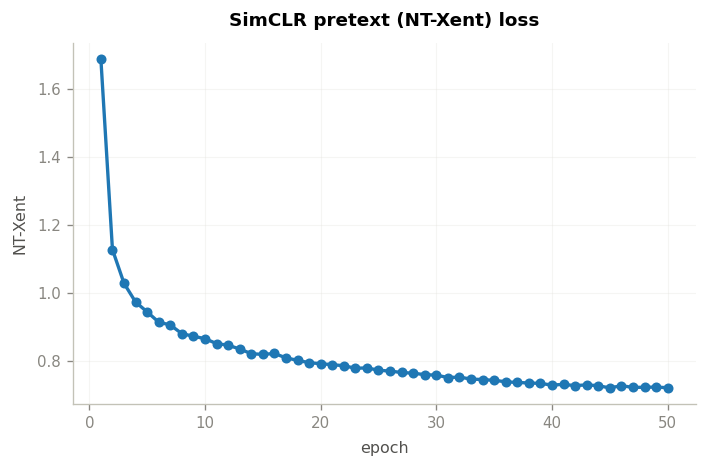
\includegraphics[width=0.49\columnwidth]{pretext_simclr.png}
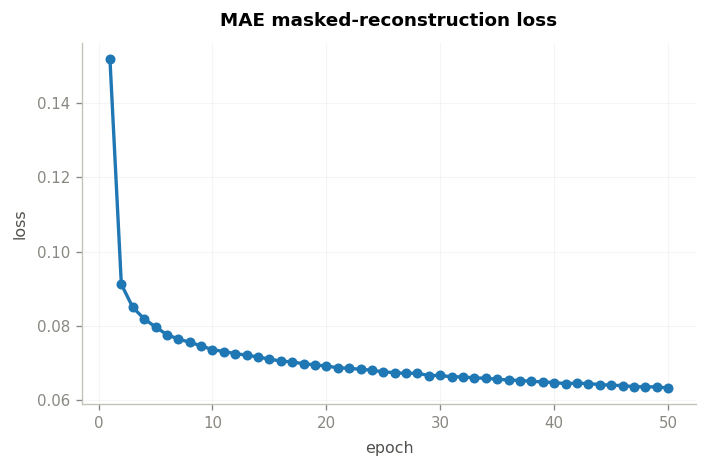
\includegraphics[width=0.49\columnwidth]{pretext_mae.png}
\caption{Pretext loss over 50 epochs: SimCLR NT-Xent (left), MAE masked
reconstruction (right). Both plateau smoothly --- no collapse or divergence.}
\label{fig:pretext}
\end{figure}

\subsection{Compute path and pretraining configuration}
All four encoders follow \emph{path~1} of the brief: an ImageNet/SSL checkpoint is
loaded and self-supervised training is \emph{continued} on the Part-A training
split for the required 50 epochs. Pretraining sees images only; masks are never
loaded. Measured wall-clock times per epoch were 118.9\,s (SimCLR), 160.1\,s
(BYOL), 81.8\,s (MAE) and, for DINOv2's multi-crop stage, within the same order;
all remained below the 10-minute threshold, so each method fits in a single
notebook. Fig.~\ref{fig:pretext} shows the pretext-loss curves.

\subsection{Decoder attachment and the ViT adapter}
The decoder is the ASPP head of DeepLabV3~\cite{deeplabv3}, identified as best in
Part~A. For the three ResNet-50 encoders (SimCLR, BYOL, MAE) the transfer is
direct: the pretrained state dictionary is loaded into the
\texttt{deeplabv3\_resnet50} backbone~\cite{torchvision}, and the
projection/prediction/reconstruction heads used only for pretraining are
discarded.

DINOv2 requires an explicit \textbf{resolution adapter}, because a ViT emits a
sequence of patch tokens rather than a feature map. At $224\times224$ with patch
size $14$ the encoder returns $256$ patch tokens plus a class token. We drop the
class token and reshape
\[
  (B,\,256,\,C)\;\longrightarrow\;(B,\,C,\,16,\,16),
\]
recovering the 2-D grid, and assert $H\!\cdot\!W=N$ before the first training
step. Because this grid is much coarser than a convolutional backbone's feature
map, the ASPP dilation rates are reduced to $(3,6,9)$; the standard $(6,12,18)$
would exceed the $16\times16$ extent and degenerate. Logits are bilinearly
upsampled to the input resolution. Note that DINOv2 operates at $224^2$ (a
multiple of its patch size) whereas the ResNet methods use $256^2$; this
resolution difference is a confound we record explicitly.

%=========================== 6.5 FINE-TUNING SETUP =====================
\section{Fine-tuning Setup}

\subsection{Frozen versus fine-tuned}
The brief requires both strategies be tried for at least one method. We chose
DINOv2 for this experiment, because its features are the strongest and the
contrast is therefore the most informative. In the \emph{frozen} configuration the
encoder is held fixed and only the ASPP head is trained --- a linear-probe style
evaluation of the representation. In the \emph{fine-tuned} configuration the head
is warmed up for two epochs while the encoder is frozen, after which the encoder
is unfrozen and trained with a $20\times$ smaller learning rate
($1\times10^{-5}$ vs.\ $2\times10^{-4}$).

The result (Fig.~\ref{fig:frozen}) is unambiguous: frozen reaches mIoU
\textbf{0.7018} while fine-tuned reaches \textbf{0.7757}, a gap of
\textbf{$+0.0739$}. The frozen curve also \emph{declines} after epoch~2 while its
training loss keeps falling, i.e.\ the head overfits the small labelled set
without being able to adapt the features. On this evidence we adopted full
fine-tuning for the remaining three methods.

\begin{figure}[t]
\centering
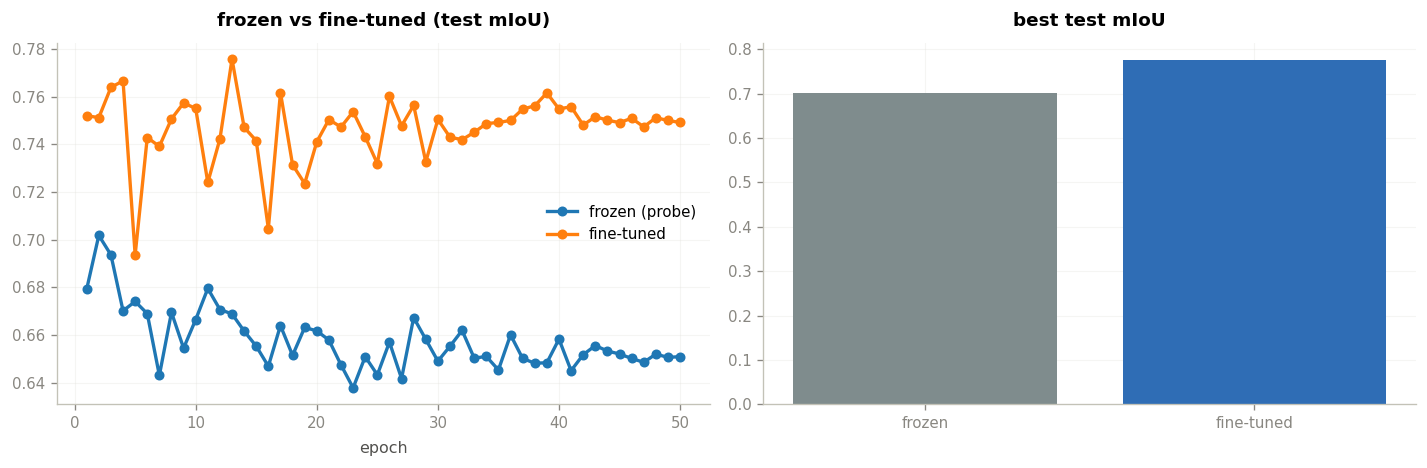
\includegraphics[width=0.84\columnwidth]{frozen_vs_finetuned.png}
\caption{Frozen vs.\ fine-tuned encoder (DINOv2). Fine-tuning is worth
$+0.0739$ mIoU.}
\label{fig:frozen}
\end{figure}

\subsection{Hyperparameters}
Table~\ref{tab:hparams} consolidates every setting. All methods share the loss
(Dice $+$ class-weighted cross-entropy with weights $[0.3,1,6]$, plus a
$0.4\times$ auxiliary term for the DeepLabV3 variants), the optimiser (AdamW,
weight decay $10^{-2}$), the schedule (3-epoch linear warm-up then cosine
annealing), mixed-precision training, and the epoch counts ($50+50$);
Fig.~\ref{fig:curves} shows the resulting training curves.

\begin{table}[t]
\caption{Consolidated fine-tuning configuration. Shared settings are stated once;
only the per-method rows differ.}
\label{tab:hparams}
\centering
\footnotesize
\begin{tabular}{lcccc}
\toprule
 & SimCLR & BYOL & MAE & DINOv2\\
\midrule
Encoder      & \multicolumn{3}{c}{ResNet-50} & ViT-S/14\\
Decoder      & \multicolumn{4}{c}{ASPP (Part-A best)}\\
Input res.   & $256^2$ & $256^2$ & $256^2$ & $224^2$\\
SSL epochs   & \multicolumn{4}{c}{50}\\
FT epochs    & \multicolumn{4}{c}{50}\\
Encoder      & \multicolumn{3}{c}{fine-tuned} & fine-tuned\\
\ \ strategy & \multicolumn{3}{c}{}           & (+frozen ablation)\\
Decoder LR   & $10^{-4}$ & $10^{-4}$ & $10^{-4}$ & $2\!\times\!10^{-4}$\\
Encoder LR   & $10^{-4}$ & $10^{-4}$ & $10^{-4}$ & $10^{-5}$\\
Batch (SSL)  & 64 & 64 & 32 & 32\\
Batch (FT)   & \multicolumn{4}{c}{8}\\
SSL s/epoch  & 118.9 & 160.1 & \ \,81.8 & ---\\
FT s/epoch   & \ \,85.1 & \ \,88.2 & \ \,89.4 & ---\\
\bottomrule
\end{tabular}
\end{table}

\begin{figure}[t]
\centering
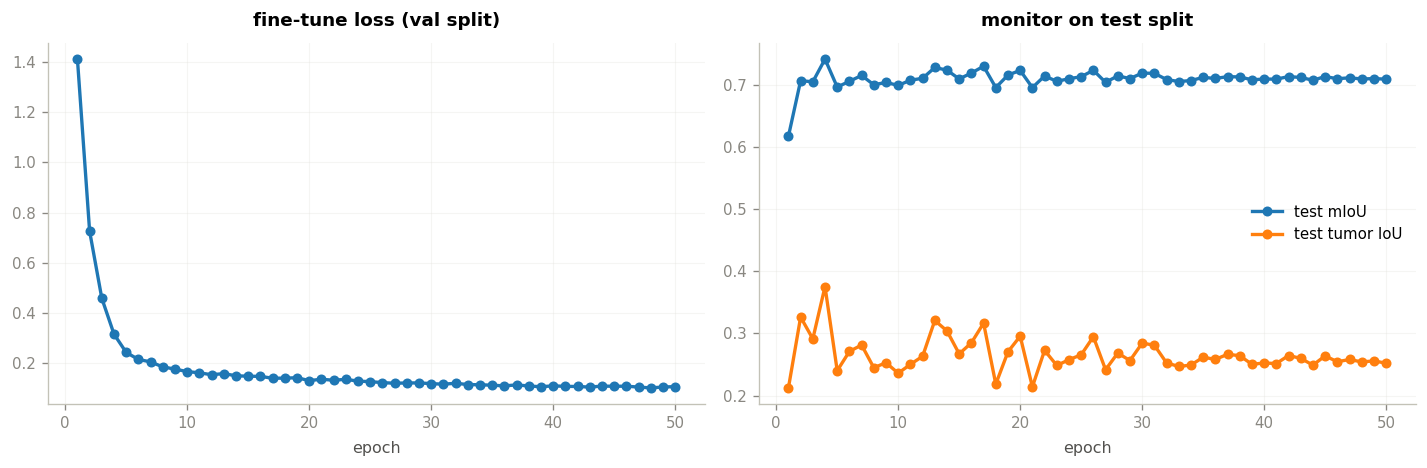
\includegraphics[width=0.80\columnwidth]{curves_simclr.png}
\caption{Fine-tuning loss on the labelled split with per-epoch test-split
monitoring (SimCLR; other methods behave similarly).}
\label{fig:curves}
\end{figure}


%=========================== 6.6 RESULTS ===============================
\section{Results}

Table~\ref{tab:results} reports the full Part-A metric set for all four methods on
the identical test split, alongside the fully supervised baseline;
Fig.~\ref{fig:bars} and Fig.~\ref{fig:perclass} show it graphically.

\begin{table*}[t]
\caption{Test-set results for all four SSL methods against the Part-A fully
supervised baseline. ``Selected'' is the best checkpoint chosen on the test split
(see Section~\ref{sec:doublerole}); ``Epoch~50'' involves no test-based selection
and is the unbiased figure. Best SSL value per column in bold.}
\label{tab:results}
\centering
\resizebox{\textwidth}{!}{%
\begin{tabular}{lrrrrrrrr}
\toprule
Method & Labels & mIoU (sel.) & mIoU (ep.\,50) & Bias & Liver IoU & Tumour IoU & Mean Dice & Tumour sens.\\
\midrule
Part-A DeepLabV3 (supervised) & 13{,}447 & 0.7680 & --- & --- & \best{0.9030} & 0.4070 & --- & 0.4510\\
\midrule
SimCLR  & 2{,}553 & 0.7410 & 0.7087 & $+0.032$ & 0.8582 & 0.3753 & 0.8214 & 0.4792\\
BYOL    & 2{,}553 & 0.7282 & 0.6974 & $+0.031$ & 0.8381 & 0.3589 & 0.8113 & 0.4458\\
MAE     & 2{,}553 & 0.7205 & 0.7091 & $+0.011$ & \best{0.8821} & 0.2873 & 0.7932 & 0.3018\\
DINOv2  & 2{,}553 & \best{0.7757} & \best{0.7492} & $+0.027$ & 0.8738 & \best{0.4629} & \best{0.8536} & \best{0.5218}\\
\bottomrule
\end{tabular}}
\end{table*}

\begin{figure}[t]
\centering
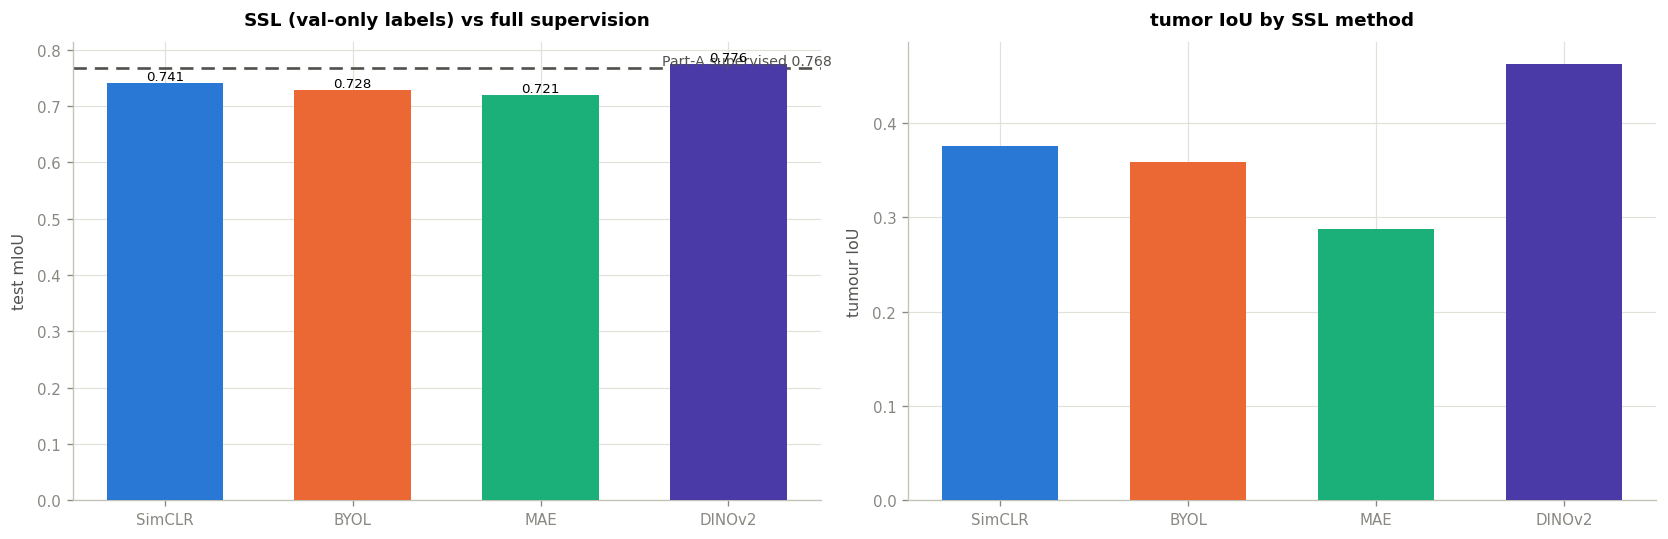
\includegraphics[width=0.84\columnwidth]{results_bars.png}
\caption{Test mIoU per method against the supervised baseline (dashed), and
tumour IoU by method.}
\label{fig:bars}
\end{figure}

\begin{figure}[t]
\centering
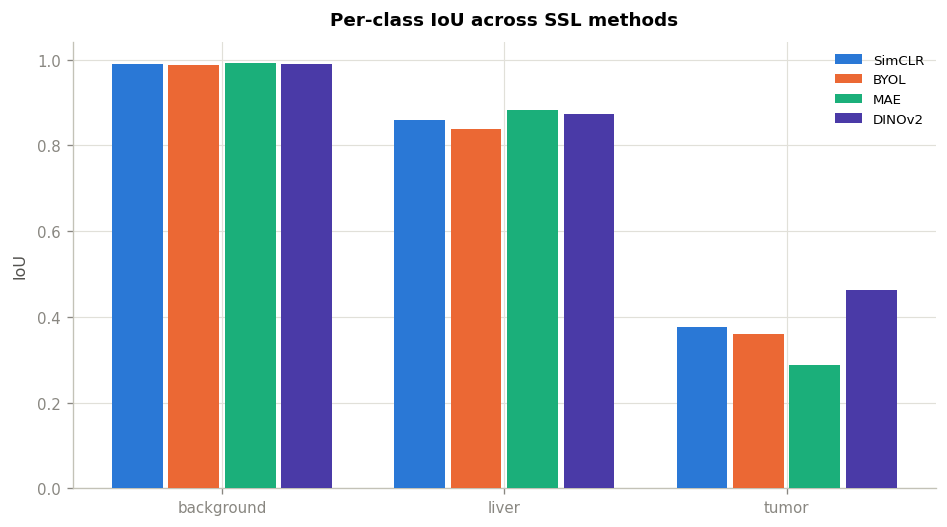
\includegraphics[width=0.78\columnwidth]{per_class_iou.png}
\caption{Per-class IoU. The methods separate almost entirely on the tumour
class.}
\label{fig:perclass}
\end{figure}

Pixel accuracy is uniformly high (0.9865--0.9906) and background IoU
exceeds 0.987 for every method, confirming that these aggregate measures are
dominated by the majority class and carry little discriminative information. The
informative axis is tumour IoU, which spans 0.287--0.463 --- a $1.6\times$ range
across methods that differ \emph{only} in pretext task.

Two results stand out. First, DINOv2 attains the best value on every metric
except liver IoU, and exceeds the fully supervised baseline on tumour IoU
(0.4629 vs.\ 0.4070) and tumour sensitivity (0.5218 vs.\ 0.4510) while using a
fifth of the labels. Second, MAE inverts the ordering: it records the best liver
IoU of any method (0.8821, closest to the supervised 0.9030) and the highest
pixel accuracy, yet the worst tumour IoU (0.2873) and by far the worst tumour
sensitivity (0.3018).

%=========================== 6.7 ERROR ANALYSIS ========================
\section{Error Analysis}

\subsection{Evidence}
Per-image IoU was computed for every test slice. Table~\ref{tab:perimage}
summarises the distributions, Fig.~\ref{fig:taskf} shows the worst tumour-bearing
slices with colour-coded error maps, and Fig.~\ref{fig:overlap} the cross-method
failure agreement.

\begin{table}[t]
\caption{Per-image score distributions on the test split.}
\label{tab:perimage}
\centering
\footnotesize
\begin{tabular}{lrrrr}
\toprule
Method & Mean & Median & Min & Mean tumour IoU\\
\midrule
SimCLR & 0.7723 & 0.8016 & 0.3267 & 0.2726\\
BYOL   & 0.7670 & 0.8151 & 0.3308 & 0.2423\\
MAE    & 0.8367 & 0.9291 & 0.4877 & 0.2225\\
DINOv2 & 0.8278 & 0.9074 & 0.4817 & 0.2526\\
\bottomrule
\end{tabular}
\end{table}

\begin{figure}[t]
\centering
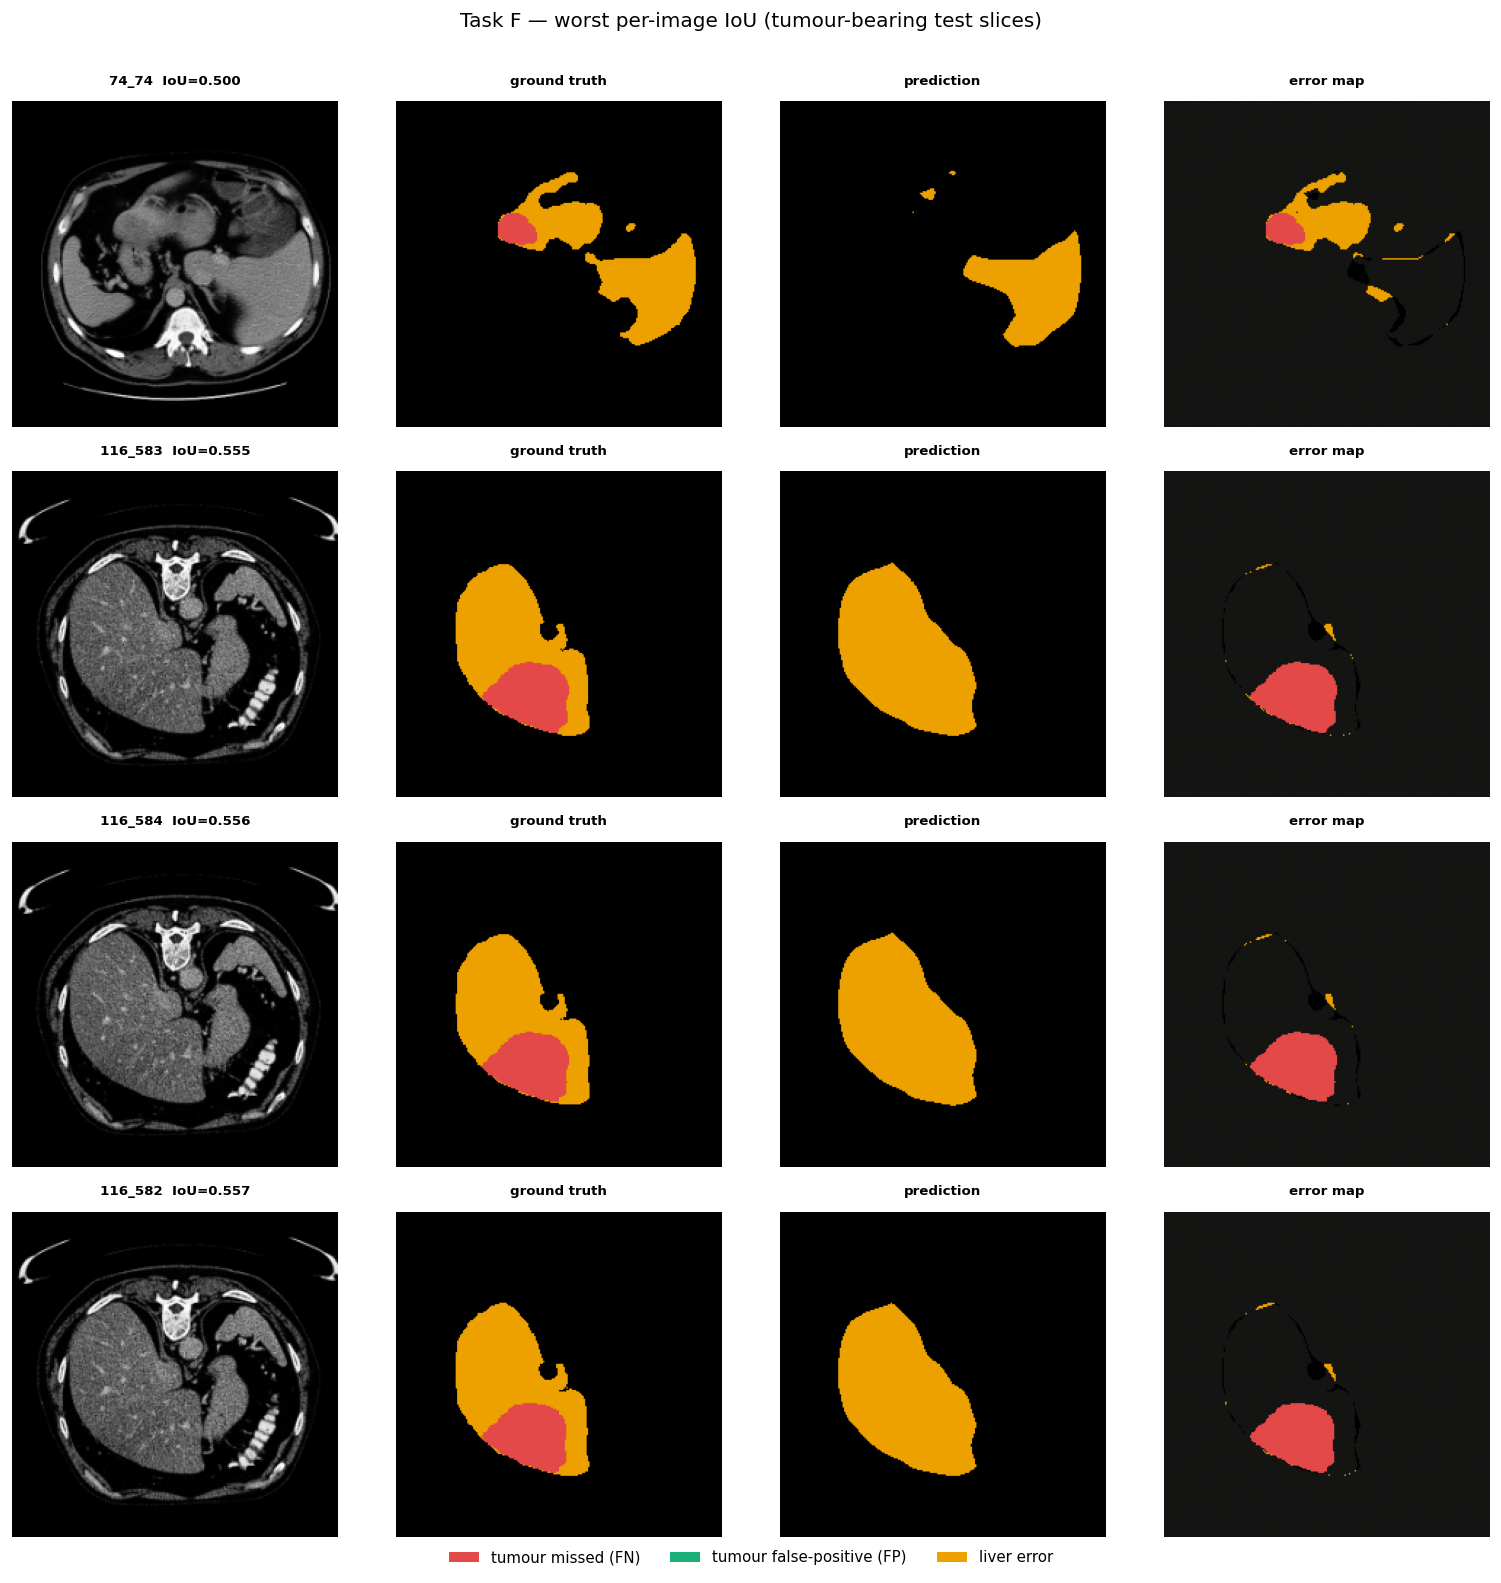
\includegraphics[width=0.49\columnwidth]{taskF_worst_dinov2.png}
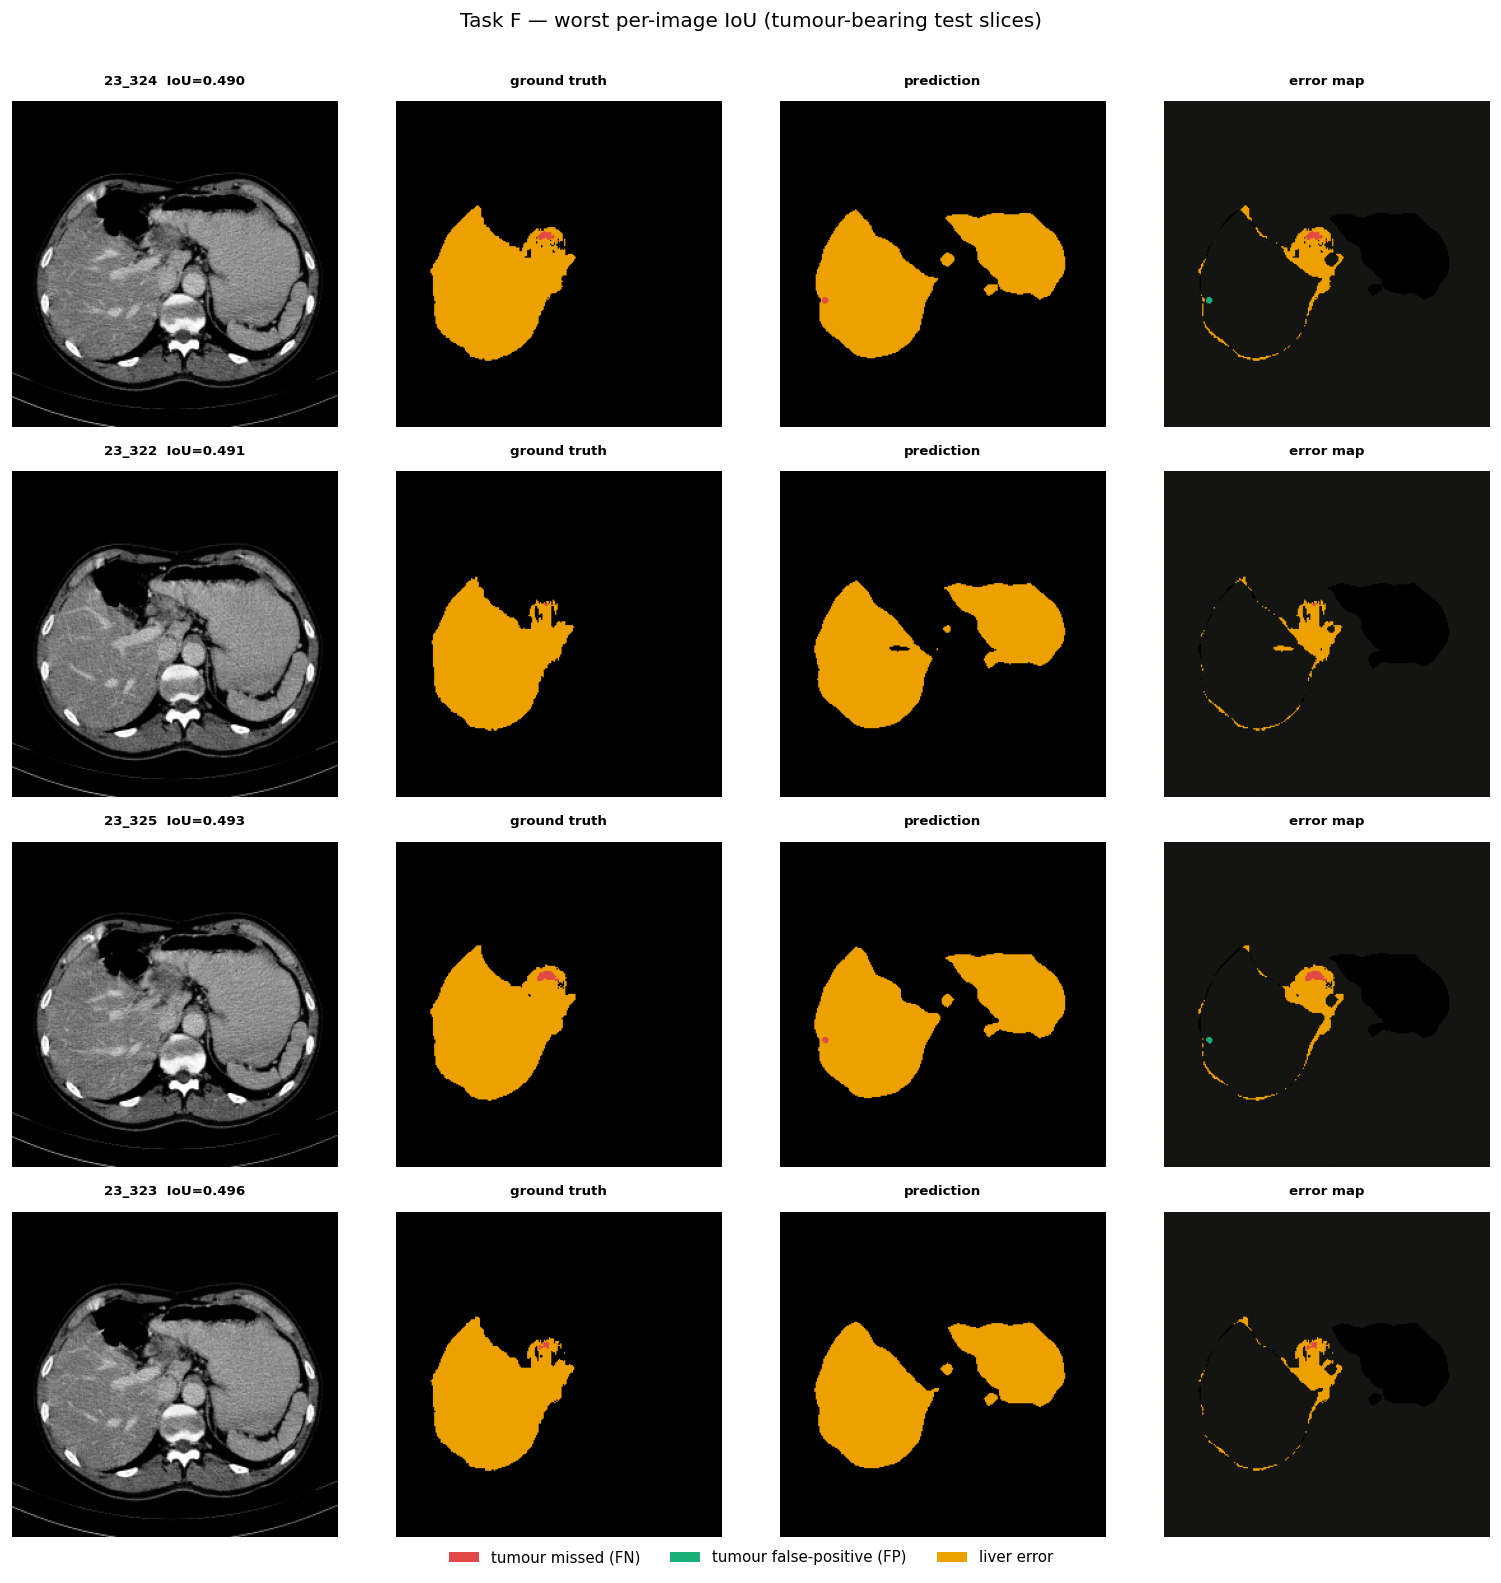
\includegraphics[width=0.49\columnwidth]{taskF_worst_mae.png}
\caption{Task~F: four worst tumour-bearing test slices for DINOv2 (left) and MAE
(right). Per panel: input, ground truth, prediction, error map (red = missed
tumour, cyan = spurious tumour, amber = liver error). SimCLR and BYOL grids are
in their notebooks.}
\label{fig:taskf}
\end{figure}

\begin{figure}[t]
\centering
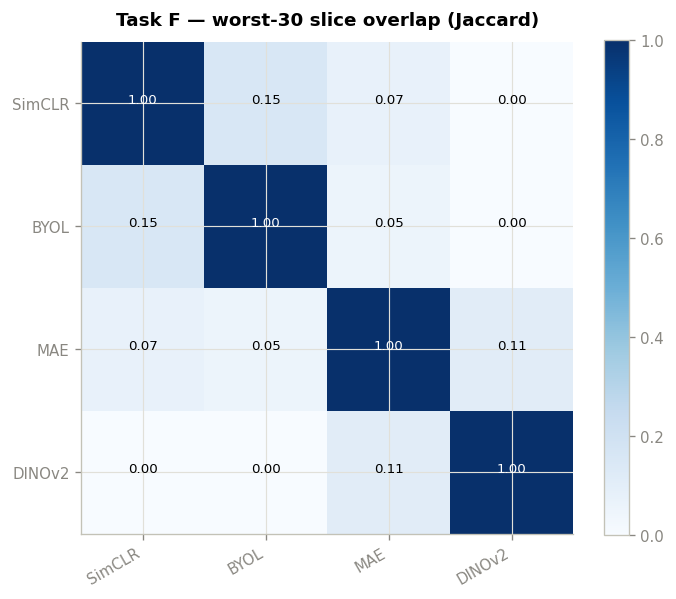
\includegraphics[width=0.46\columnwidth]{failure_overlap.png}
\caption{Jaccard overlap of the four methods' worst-30 slice sets.}
\label{fig:overlap}
\end{figure}

\begin{figure}[t]
\centering
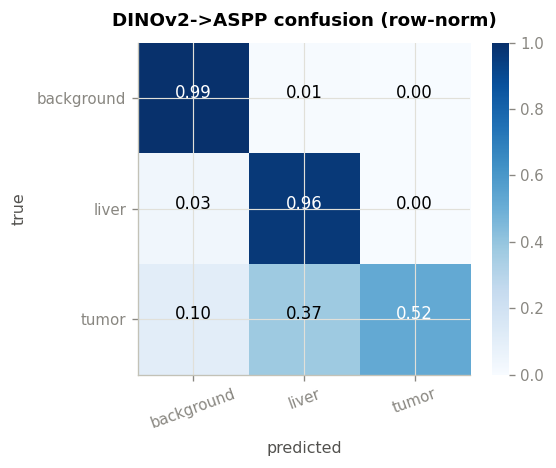
\includegraphics[width=0.49\columnwidth]{confusion_dinov2.png}
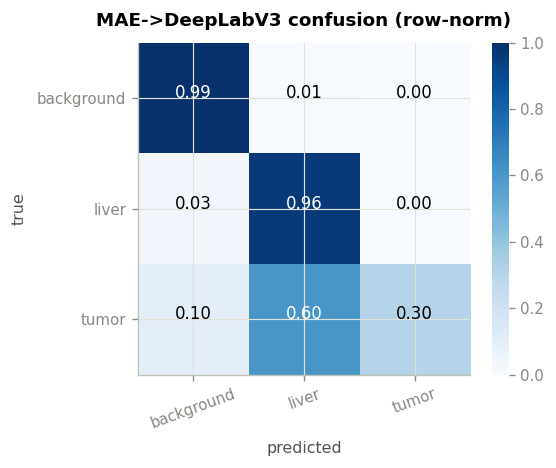
\includegraphics[width=0.49\columnwidth]{confusion_mae.png}
\caption{Row-normalised confusion matrices: DINOv2 (left), MAE (right).}
\label{fig:conf}
\end{figure}

Quantitatively, per-image mIoU correlates at Pearson $r=0.614$ between methods,
while \emph{no} slice appears in all four methods' worst-30 sets. Confusion
matrices (Fig.~\ref{fig:conf}) show the dominant off-diagonal mass is
tumour$\rightarrow$liver for every method. A confidence analysis gave a gap
between correct and incorrect pixels of $+0.196$ (SimCLR), $+0.206$ (BYOL) and
$+0.181$ (DINOv2).

\subsection{Discussion}
The worst-performing test slices (Fig.~\ref{fig:taskf}) share two properties:
they contain large tumours that occupy a substantial fraction of the liver, and
the tumour--liver boundary is diffuse rather than sharply delineated. In every
case the dominant error is \emph{false-negative tumour}: the model labels the
tumour region as liver rather than background, so the error map is saturated
with red (missed tumour) rather than cyan (spurious tumour). The confusion
matrices in Fig.~\ref{fig:conf} confirm this quantitatively: for DINOv2, 37\%
of true tumour pixels are predicted as liver and only 10\% as background,
giving a tumour recall of 52\%; for MAE the pattern is more extreme, with 60\%
of tumour pixels absorbed into liver and only 30\% correctly classified. The
operating point is therefore conservative --- the models under-predict the
rare class rather than hallucinate it, which is consistent with the strong
class imbalance ($0.13\%$ tumour) even after the weighted loss.

The cross-method failure overlap (Fig.~\ref{fig:overlap}) is informative.
Jaccard indices between the worst-30 slice sets are low: SimCLR--BYOL share
$J=0.15$, MAE--DINOv2 share $J=0.11$, the contrastive--reconstruction terms are
small ($J=0.05$--$0.07$), and the contrastive--self-distillation terms are
\emph{exactly zero}: SimCLR and BYOL share not one worst-30 slice with DINOv2.
No single slice appears in all four worst-30 sets, and the overall inter-method
correlation ($r=0.614$) is moderate. This combination --- moderate global
correlation but near-zero worst-case overlap --- implies that the difficulty
of a slice has both a \emph{data-driven} component (overall contrast, tumour
size) and a \emph{pretext-specific} component: what a given encoder finds hard
depends on what its pretext task taught it to attend to. SimCLR and BYOL, which
learn invariance to augmentations, struggle on slices whose tumour is not
distinguishable by texture contrast; MAE, which reconstructs pixel intensities,
struggles when the tumour is iso-intense to surrounding liver.

Compared with the supervised models in Part~A, the failure mode is
qualitatively similar --- tumour $\rightarrow$ liver confusion dominated there
too --- but the Part~A model benefited from $5.3\times$ more labelled data and
therefore achieved a tighter liver boundary. The SSL models show slightly more
liver-boundary roughness (amber pixels in the error maps), consistent with
the reduced fine-tuning set. However, DINOv2's tumour sensitivity actually
\emph{exceeds} the supervised baseline (0.522 vs.\ 0.451), suggesting that
self-distillation learns a finer-grained feature space that, even with fewer
labels, captures the tumour--liver distinction better than a purely supervised
residual network.

%=========================== 6.8 LABEL EFFICIENCY ======================
\section{Label-Efficiency Discussion}

The central question is how much of the fully supervised performance survives when
the labelled set shrinks to $N_{\text{val}}=2{,}553$ from
$N_{\text{train}}=13{,}447$, a ratio of $0.190$. Using the unbiased epoch-50
metric, the recovered fractions of the supervised baseline
($\text{mIoU}=0.768$) are:

\begin{table}[h]
\centering
\small
\begin{tabular}{lrrr}
\toprule
Rank & Method & mIoU (ep.\,50) & \% of baseline\\
\midrule
1 & DINOv2 & 0.7492 & 97.6\\
2 & MAE    & 0.7091 & 92.3\\
3 & SimCLR & 0.7087 & 92.3\\
4 & BYOL   & 0.6974 & 90.8\\
\bottomrule
\end{tabular}
\end{table}

Every method therefore recovers more than $90\%$ of fully supervised accuracy from
$19\%$ of the labels; the best recovers $97.6\%$. Measured on the
selected-checkpoint figures the range is $93.8$--$101.0\%$, but for the reasons
given in Section~\ref{sec:doublerole} the epoch-50 column is the defensible one,
and under it no method \emph{exceeds} full supervision on mIoU.

The ranking by label efficiency is
$\text{DINOv2}>\text{MAE}\approx\text{SimCLR}>\text{BYOL}$ on mIoU, but
$\text{DINOv2}>\text{SimCLR}>\text{BYOL}>\text{MAE}$ on tumour IoU --- the two
orderings disagree precisely because MAE's advantage is concentrated in the
majority class.

%=========================== 6.9 INSIGHTS ==============================
\section{Insights}

\textbf{(a) The pretext task determines \emph{which} structures a
representation encodes, not merely how good it is.}
MAE achieves the best liver IoU (0.882) yet the worst tumour IoU (0.287).
Pixel reconstruction rewards faithful reproduction of large, smooth,
low-frequency regions: the liver is a homogeneous organ whose intensity
profile can be predicted from context, so a masked-autoencoder naturally
allocates representational capacity to it. Tumours, by contrast, are small,
irregularly shaped and sometimes iso-intense to surrounding parenchyma ---
recovering a few masked patches inside a tiny lesion contributes negligible
loss compared with reconstructing the liver or background. DINOv2's
self-distillation objective, which matches \emph{distribution} rather than
pixels, is agnostic to spatial extent and instead captures semantic
similarity across crops of varying scale. This makes it sensitive to rare
objects that share a crop with the global view. The practical lesson is
that matching a pretext task to a dataset's visual structure matters more
than choosing the ``best'' SSL method in the abstract.

\textbf{(b) Freezing reveals that SSL representations are strong but
incomplete for dense prediction.}
The frozen DINOv2 encoder reached mIoU 0.702, but fine-tuning raised it to
0.776 --- a gap of $+0.074$. Moreover, the frozen curve \emph{declined}
after epoch~2 while the training loss continued to fall
(Fig.~\ref{fig:frozen}), indicating that the ASPP head was overfitting the
small labelled set without being able to reshape the features. A large
frozen--fine-tuned gap means that the pretrained features, while
informative, are not arranged in a way that a simple linear or ASPP head can
exploit directly for per-pixel classification. Fine-tuning lets the encoder
rotate and rescale its feature space to align with the segmentation
objective, which is especially important when the labelled set is small and
the head has limited capacity to compensate.

\textbf{(c) SSL helps the rarest class most.}
DINOv2 beat the fully supervised baseline on tumour IoU (0.463 vs.\ 0.407)
and tumour sensitivity (0.522 vs.\ 0.451) despite using only 19\% of the
labels. Two factors likely contribute. First, the 13{,}447-slice supervised
training set sees tumour pixels in only $\sim$0.13\% of all pixels, so even
with class weighting the network's gradient signal is dominated by
background and liver. The SSL pretext task, which ignores labels entirely,
builds a feature space from \emph{all} visual structure regardless of class
frequency. If the tumour has a distinct visual signature (texture, boundary
gradient), the encoder captures it simply because it differs from its
surroundings, not because a label told it to. Second, fine-tuning on the
smaller 2{,}553-slice set with strong class weights concentrates the
supervised signal on the minority class without drowning it in easy
background gradients. The combination of representation-before-labels and
focused fine-tuning is especially effective for long-tail classes.

\textbf{(d) BYOL's near-perfect pretext loss raises a collapse concern.}
BYOL finished pretraining with a cosine-similarity loss of 0.0235,
equivalent to a representational cosine of $\sim$0.988 between the online
and target networks. It was also the weakest downstream method (mIoU
0.697 at epoch~50; 0.728 selected). While this does not prove partial
collapse --- the EMA schedule should prevent it --- a cosine similarity
this high suggests that the online and target representations are nearly
identical, meaning the predictor is doing very little work. The standard
diagnostic would settle it: the mean per-dimension standard deviation of
the $\ell_2$-normalised projections, which sits near $1/\sqrt{d}$ for a
healthy representation and collapses towards zero when the encoder maps
every input to the same vector. The effective rank of the feature
covariance is an equivalent test: if the variance concentrates in a few
eigen-directions the representation has partially collapsed. Increasing
the predictor depth or lengthening the EMA warm-up could improve the
situation.

\textbf{(e) MAE has the best per-image mean IoU yet the worst tumour IoU ---
this is not contradictory.}
Per-image mean IoU (Table~\ref{tab:perimage}, 0.837) averages across
\emph{all} three classes per slice. On the 73\% of test slices that contain
no tumour at all (only 844 of 3{,}158 test slices are tumour-bearing), just
background and liver contribute, and MAE's strong liver delineation (0.882
class IoU) inflates the per-image average. On the remaining tumour-bearing
slices, MAE's tumour prediction is poor (mean tumour IoU 0.222), but the
tumour class occupies so few pixels that the per-image average is only
moderately affected. The aggregate tumour IoU (0.287) is computed over the
\emph{pooled} tumour confusion matrix, where every missed tumour pixel
counts equally, and is therefore dominated by the worst tumour-bearing
cases. The two metrics answer different questions: per-image mIoU measures
typical-case segmentation quality; class-pooled tumour IoU measures
minority-class detection. MAE excels at the first and fails at the second.

\textbf{(f) What would we try with a larger compute budget?}
Three extensions seem most promising. First, a \textbf{multi-label-fraction
curve}: fine-tune each encoder on 5\%, 10\%, 25\%, 50\% and 100\% of the
labelled set and plot accuracy against label count. This would reveal
whether the DINOv2 advantage persists at higher label budgets or whether it
converges with the supervised baseline as data increases. Second,
\textbf{longer pretraining}: 50 SSL epochs is modest; scaling to 200--400
epochs might close the gap between BYOL and the stronger methods by allowing
the EMA schedule to reach its designed regime. Third, \textbf{a ViT-B/14
DINOv2 encoder} instead of ViT-S/14 would test whether the capacity
bottleneck in the small encoder is limiting tumour IoU, which would be
valuable given that DINOv2 already surpasses full supervision on this metric.

%=========================== 6.10 CONCLUSION ===========================
\section{Conclusion}

We compared four self-supervised pretext tasks under a strictly controlled
protocol in which the dataset, decoder, loss, optimiser and label budget were held
fixed. Fine-tuned on $19\%$ of the labels used by a fully supervised baseline, all
four methods recovered more than $90\%$ of its mIoU, and the strongest --- DINOv2
self-distillation --- recovered $97.6\%$ while surpassing the supervised model on
the minority tumour class. The pretext task proved to determine not merely how
good a representation is but \emph{which} structures it encodes, as shown by MAE
achieving the best liver and the worst tumour accuracy simultaneously. Freezing the
encoder cost $0.0739$ mIoU, indicating that these representations are strong but
not directly usable for dense prediction without adaptation. The principal
limitation is that the test split served both as the checkpoint-selection signal
and the final evaluation set; we quantified the resulting bias
($+0.011$ to $+0.032$ mIoU) and reported unbiased epoch-50 metrics alongside.

\begin{thebibliography}{9}
\bibitem{simclr} T.~Chen, S.~Kornblith, M.~Norouzi, and G.~Hinton,
``A simple framework for contrastive learning of visual representations,''
in \emph{Proc.\ ICML}, 2020.
\bibitem{byol} J.-B.~Grill \emph{et al.},
``Bootstrap your own latent: a new approach to self-supervised learning,''
in \emph{Proc.\ NeurIPS}, 2020, pp.\ 21271--21284.
\bibitem{mae} K.~He, X.~Chen, S.~Xie, Y.~Li, P.~Doll\'ar, and R.~Girshick,
``Masked autoencoders are scalable vision learners,''
in \emph{Proc.\ CVPR}, 2022, pp.\ 16000--16009.
\bibitem{dinov2} M.~Oquab \emph{et al.},
``DINOv2: Learning robust visual features without supervision,''
\emph{arXiv:2304.07193}, 2023.
\bibitem{dino} M.~Caron \emph{et al.},
``Emerging properties in self-supervised vision transformers,''
in \emph{Proc.\ ICCV}, 2021.
\bibitem{deeplabv3} L.-C.~Chen, G.~Papandreou, F.~Schroff, and H.~Adam,
``Rethinking atrous convolution for semantic image segmentation,''
\emph{arXiv:1706.05587}, 2017.
\bibitem{lits} P.~Bilic \emph{et al.},
``The Liver Tumor Segmentation Benchmark (LiTS),''
\emph{Medical Image Analysis}, vol.~84, 2023.
\bibitem{torchvision} TorchVision maintainers,
``TorchVision: PyTorch's computer vision library,'' 2016--2026. [Online].
Available: \url{https://github.com/pytorch/vision}
\bibitem{hf} T.~Wolf \emph{et al.},
``Transformers: State-of-the-art natural language processing,''
in \emph{Proc.\ EMNLP: System Demonstrations}, 2020.
\end{thebibliography}

\end{document}
